\documentclass[runningheads]{llncs}
\usepackage[utf8]{inputenc}

\usepackage{graphicx}
\usepackage{amsmath}
\usepackage{amssymb}
\usepackage{arydshln}
\usepackage{xcolor,ulem}

\usepackage{wrapfig}

% Used for displaying a sample figure. If possible, figure files should
% be included in EPS format.
%
% If you use the hyperref package, please uncomment the following line
% to display URLs in blue roman font according to Springer's eBook style:
% \renewcommand\UrlFont{\color{blue}\rmfamily}

\setlength{\parskip}{0cm}
\setlength{\parindent}{1em}

\newcommand{\reals}{\mathbb{R}}

\newcommand{\comment}[3]{{\color{#1} {\bf #2 :} #3}}
%\newcommand{\comment}[3]{}  % suppress comments
\newcommand{\kui}[1]{\comment{blue}{Kui}{#1}}
\newcommand{\yoav}[1]{\comment{purple}{Yoav}{#1}}
\renewcommand{\beth}[1]{\comment{red}{Beth}{#1}}
\newcommand{\david}[1]{\comment{cyan}{David}{#1}}

\renewcommand\floatpagefraction{.99}
\renewcommand\topfraction{.99}
\renewcommand\bottomfraction{.99}
\renewcommand\textfraction{.1}   
\setcounter{totalnumber}{50}
\setcounter{topnumber}{50}
\setcounter{bottomnumber}{50}
\setlength{\abovecaptionskip}{0pt}
\setlength{\belowcaptionskip}{0pt}

\title{Towards explainable semi-automated Neuroanatomy}
\author{Kui Qian, Zhongkai Wu, Beth Friedman, David Kleinfeld, Yoav Freund}
\date{January 2022}

\begin{document}

\maketitle

\begin{abstract}
  A fundamental goal of neuroanatomy is the identification of brain
  structures.  Manual identification of structures is based on the
  spatial distribution of cell shape, size, orientation and density.
  With new technology it is possible to image entire brains at high
  resolution.  However, manual identification of structures in these
  massive datasets is prohibitively time consuming.  We present a
  machine learning method for automatic detection of brain
  structures. Our approach is based on diffusion maps, in combination
  with hand-picked features, and Adaboost for combining the
  features. Our method is robust against brain to brain variation and
  details of neuronal staining.  Our method produces structure
  detections together with their explanation. This that the human
  anatomist and the computer interact to improve the detection of
  structures and the addition of new structures.
  
  %We translate each cell image into a feature vector that
  %includes aspect ratio, orientation and area, as well as additional
  %features derived using a graph Laplacian. The algorithm uses the
  %statistical distribution of these features vectors to identify brain
  %structures.
\end{abstract}

\section{Main}

\yoav{A comment by yoav}, 
\beth{a comment by beth},
\david{a comment by david}

\begin{enumerate}
\item {\bf Summary:} We propose a system for assisting a neuroanatomist
  with tasks of detecting and localizing structures and cells within the mouse brainstem. Our system supports two tasks, the first is localizing the center of mass of structures in the brain-stem. The second is localizing marked cells.
  
  Our system takes as input high-resolution images of aligned
  sections and anatomical annotations generated manually that are used as training data for a machine learning (ML) algorithm. The ML algorithm 
  
  \yoav{working here}
  Each detection is assigned a confidence. High
  confidence structures are associated with a visual explanation.
  We demonstrate that for both tasks our system is able
  to accurately and confidently localize most of the targets, thereby
  significantly decreasing the anatomist work load.

\item {\bf Significance for Neuroanatomy}
Does not have to be very detailed. Target audience is ML.
\begin{itemize}
\item Importance and History
\item Manual detection of brain structures has two major drawbacks, the first is the amount of time needed by an anatomist. The second is inconsistencies between anatomists. Automatic detection has the potential of reducing the time and improving the consistency for this task.
\item Challenges: Variability of images
    \begin{itemize}
        \item biology: animal to animal, gender, generally alien across species, transgenic (differentions to genome due to gene expression)
        \item technical: staining, sectioning (mechanical, optical)
    \end{itemize}
  \end{itemize}
  
\subsubsection{Explainable AI} The traditional vision for AI is to design
an algorithm which can perform as well as, and hopefully better than
an expert human. The explosive growth in machine-learning based AI is
evidence that this vision is becoming a reality.

Indeed, in some domains, such as the game of go \cite{} deep neural
networks have achieved super-human capabilities. On the other hand, in
domains that involve images of organic phenomena, expert-level
experience is hard to achieve. This stems from two main reasons.

The first reason is the high variability of the data. Images
of brain slices vary significantly because of animal to animal
variability and because of variability in the preparation process,
including staining, sectioning and imaging. This variability between
domains has become an important direction of deep learning under
titles such as domain adaptation~\cite{wang2018deep} and transfer
learning~\cite{weiss2016survey}. The research in this area is very
active, however, the conclusion from meta-analysis efforts such as
iWilds~\cite{}, \david{please add an explaination that iWilds enforces the notion that changes in distribution statistics will confound results} indicate that the problem remains a difficult one.

The second reason is the variability between labelers. In other words,
different experts, working independently, sometimes provide different
labels. This is especially the case when the label is an annotation
such as the boundary of a structure. Data about such variability is
not easy to come by. Significant disagreement levels are well known in
medical diagnostics and are studied under the title ``inter-rater
variability''~\cite{gellhorn2013inter}. As can be expected, the level
of disagreement varies from task to task. Some annotation tasks are
``easy'' and result in annotations that are very similar, while others
are ``hard'' and result in highly varying annotations.

Our system is based on the distinction between easy and hard
instances. With each detection it associates a numeric measure of
``confidence''.


in the labeling between different anatomists. When the variation
between anatomist is large the meaning of ``better than human''
becomes less clear.


black-box approaches to computer vision
are often sensitive to small changes in the way images are acquired.

In the context of section based neuroanatomy such changes include
variability in staining, sectioning and slicing.
vary.

\subsubsection{Cell based approach}  Most CNN-based method of image
analysis are based on the concept of a sliding window. This implies
that an
y explanation provided by the CNN is based on the content of one or more windows. Windows need to be large enough to capture the image statistics. This means that a typical window contains 10-100 cells.
On the other hand, anatomist base their analysis on cytoarchitecture, which, in turn, is based on the shapes of individual cells and the relationshp between them. This makes it harder for the anatomist to understand the decisions of the detector.

To remedy this problem and make the detections explainable, we use individual cells as our basic unit. 
\end{enumerate}

\section{System design}

The trained system is a collection of structure detectors. Each structure is a known anatomical entity. 
\begin{wrapfigure}{R}{0.6\textwidth}
\centering
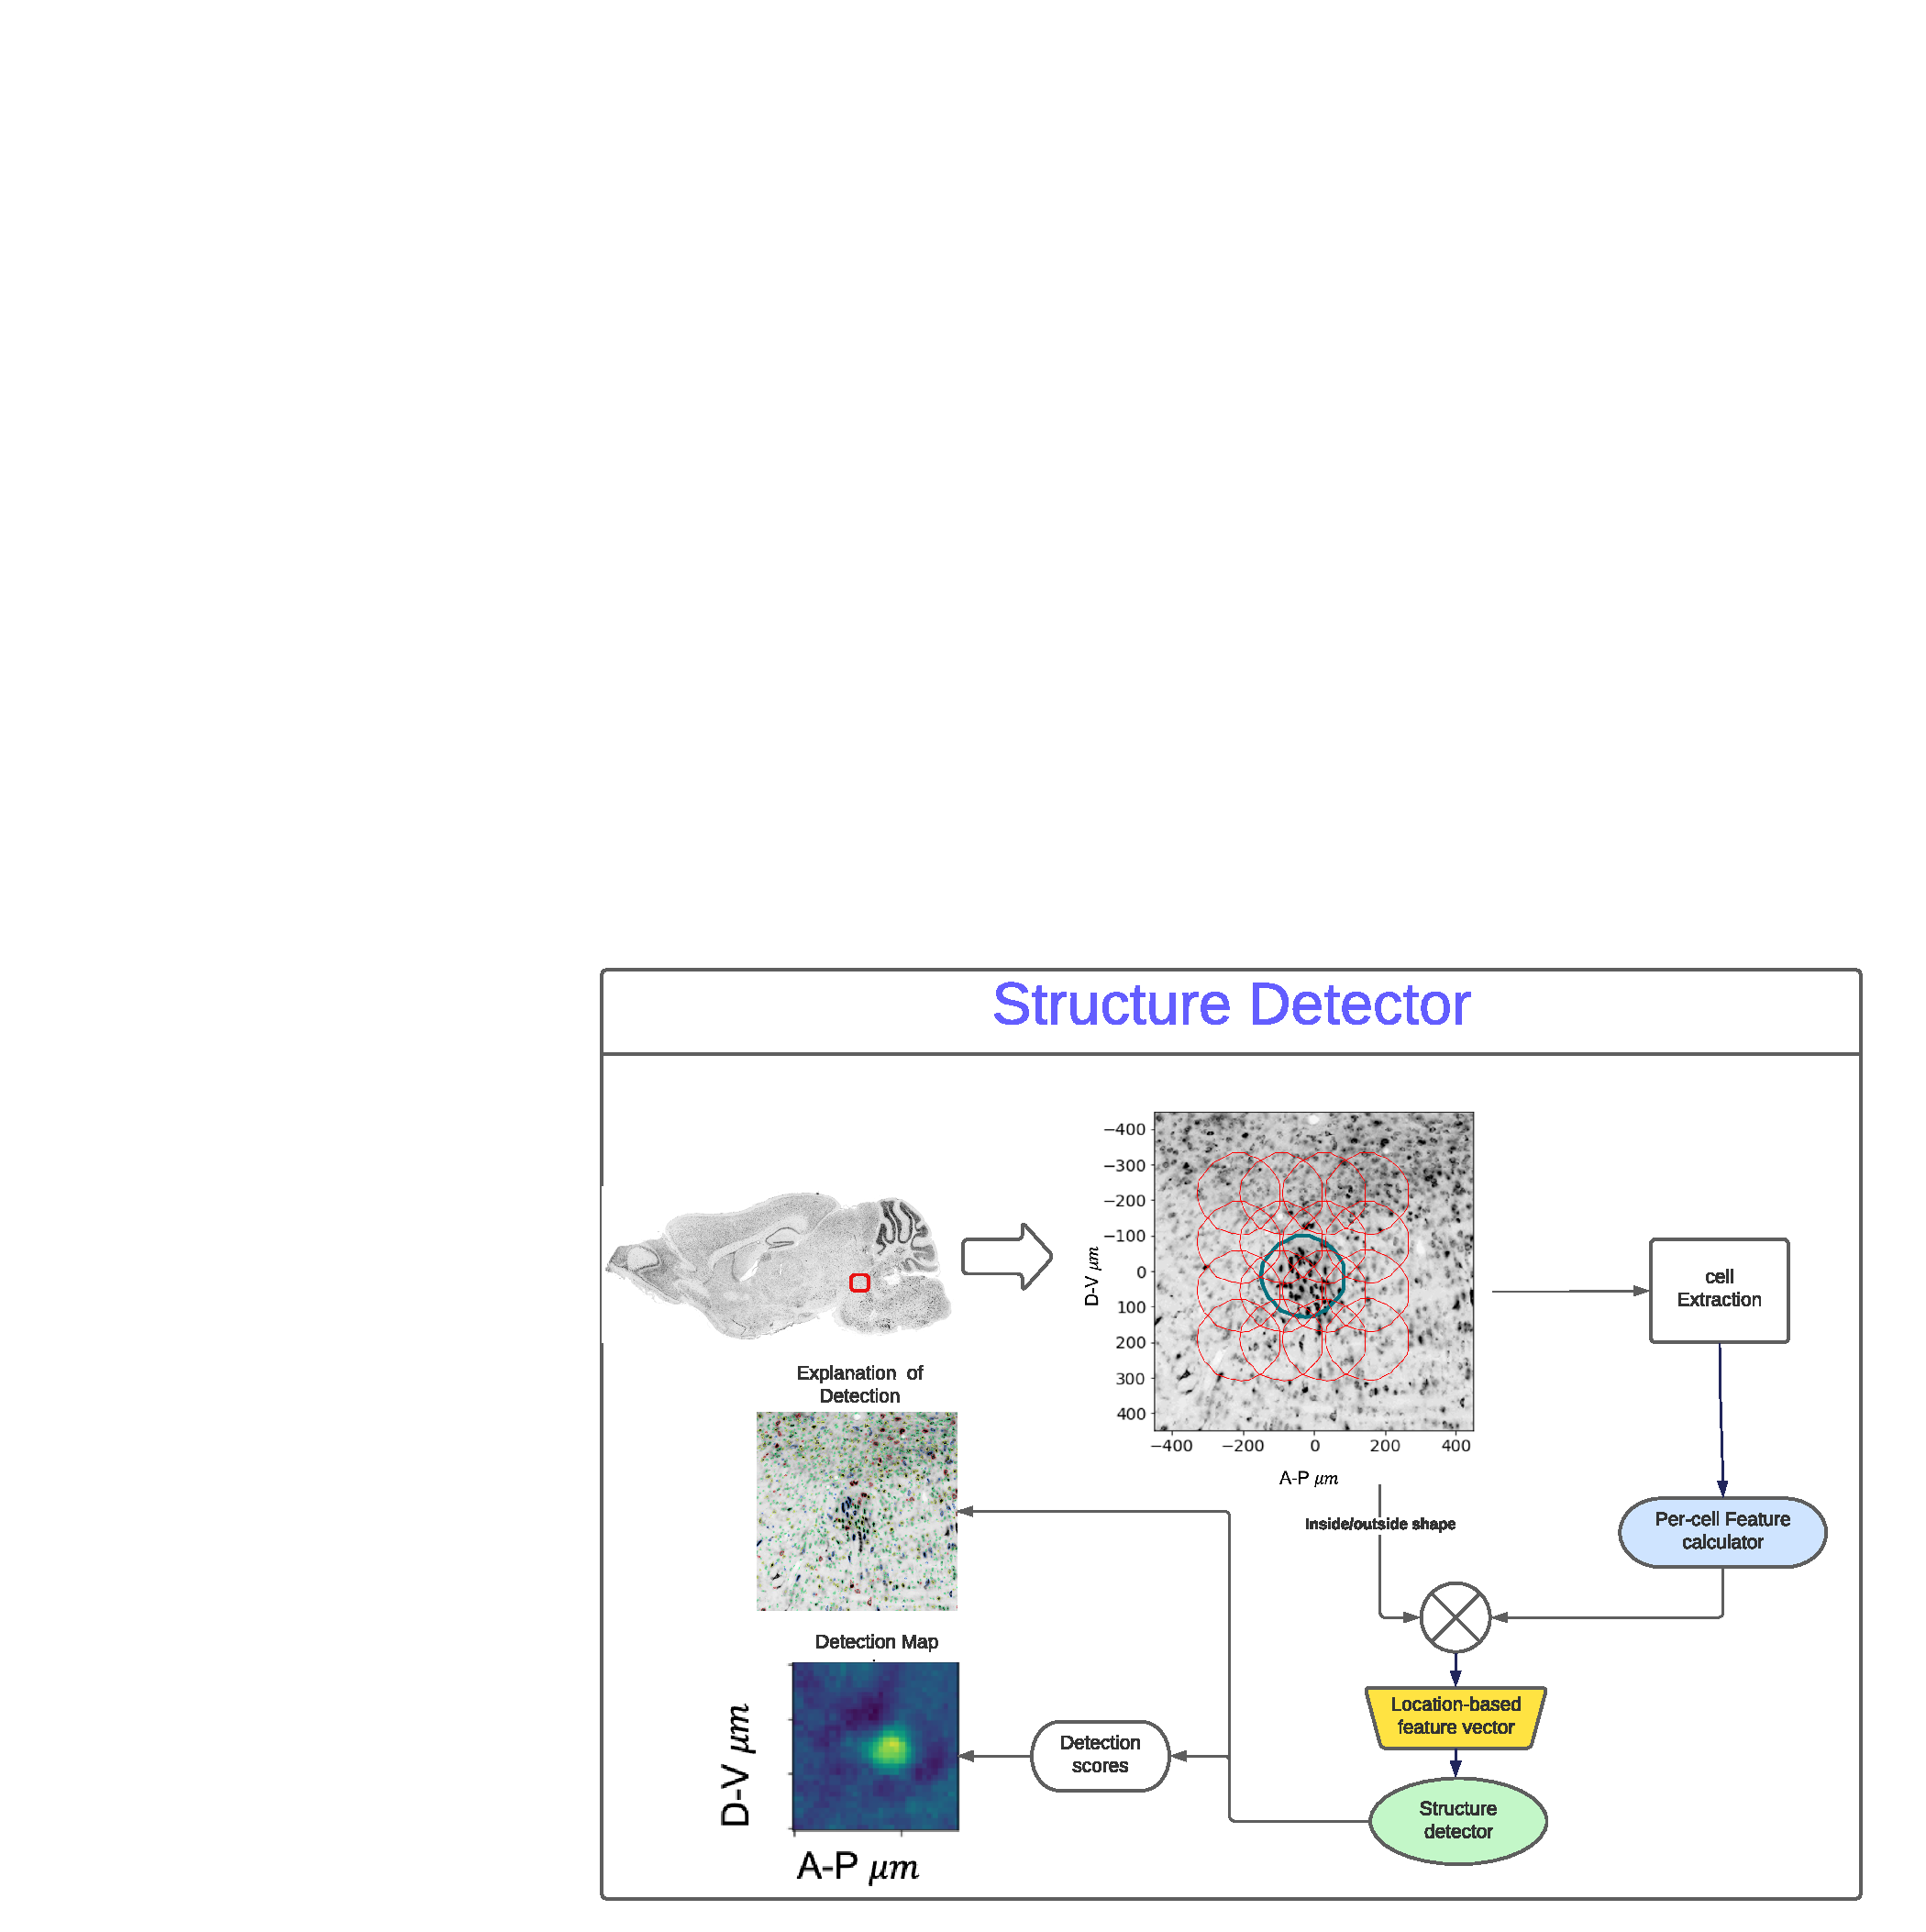
\includegraphics[width=0.5\textwidth]{figures/detection.pdf}
\caption{Detection \label{fig:detect}}
\end{wrapfigure}


The overall design of the system is shown in Figure xxx. The system can be partitioned into two parts. The training algorithm and the trained detector.

\subsection{System Inputs}
To train the detectors we combine three sources of information:
\begin{itemize}
    \item {\bf Images of aligned sections:} The Nissl images of XX brains are the primary information source. They are also by far the largest at XXX GB per brain.
    \item {\bf The Atlas} is a representation of the shape of each structure and the relative locations of the structures. The atlas was constructed through a concensus ....
    \item {\bf COMs for individual brains:} For XX brains we had an anatomist locate the COM ....
\end{itemize}

\subsection{System components}

\begin{enumerate}
\item{\bf Cell extraction and shape parametrization}
An image of a single cell is typically around 50$\times$50 pixels, or a 2500 dimensional vector. The dimension of this representation is too high for effective machine learning. We therefor seek a dimensionality reduction mapping. This mapping consists of three parts:
\begin{enumerate}
    \item {\bf Normalization:} We normalize the image of the cell in three ways. We 
    shift the grey-levels so that the mean is XXX, scale the grey levels so that the standard deviation is YYY, and rotate the image so that the long axis of the cell is in angle zero. The three parameters associated with the normalizations define three features.
    \item {\bf Standard shape features}: we use the Hu features: x,y,z...
    \item{ \bf  Diffusion maps}: Diffusion Mapping~\cite{Belkin,
        Coifman} is a non-linear dimensionality reduction method that
      is based on a graphical representation of the data and on the
      Laplace operator on graphs.
      \end{enumerate}
\end{enumerate}
      \subsubsection{ Characterizing Cytoarchitecture} uses Difference between the CDFs for inside and outside of each structure (based on manually annotated structure boundaries). 
\subsubsection { Structure detectors} Combine the difference-of-CDF
features using boosted trees (XGBoost). Each structure has a
corresponding detector.

\subsubsection { Structure detection confidence} The confidence of structure
  detections is measured by the prediction margin and by the sharpness
  of the detection peak.
\begin{wrapfigure}{R}{0.65\textwidth}
\centering
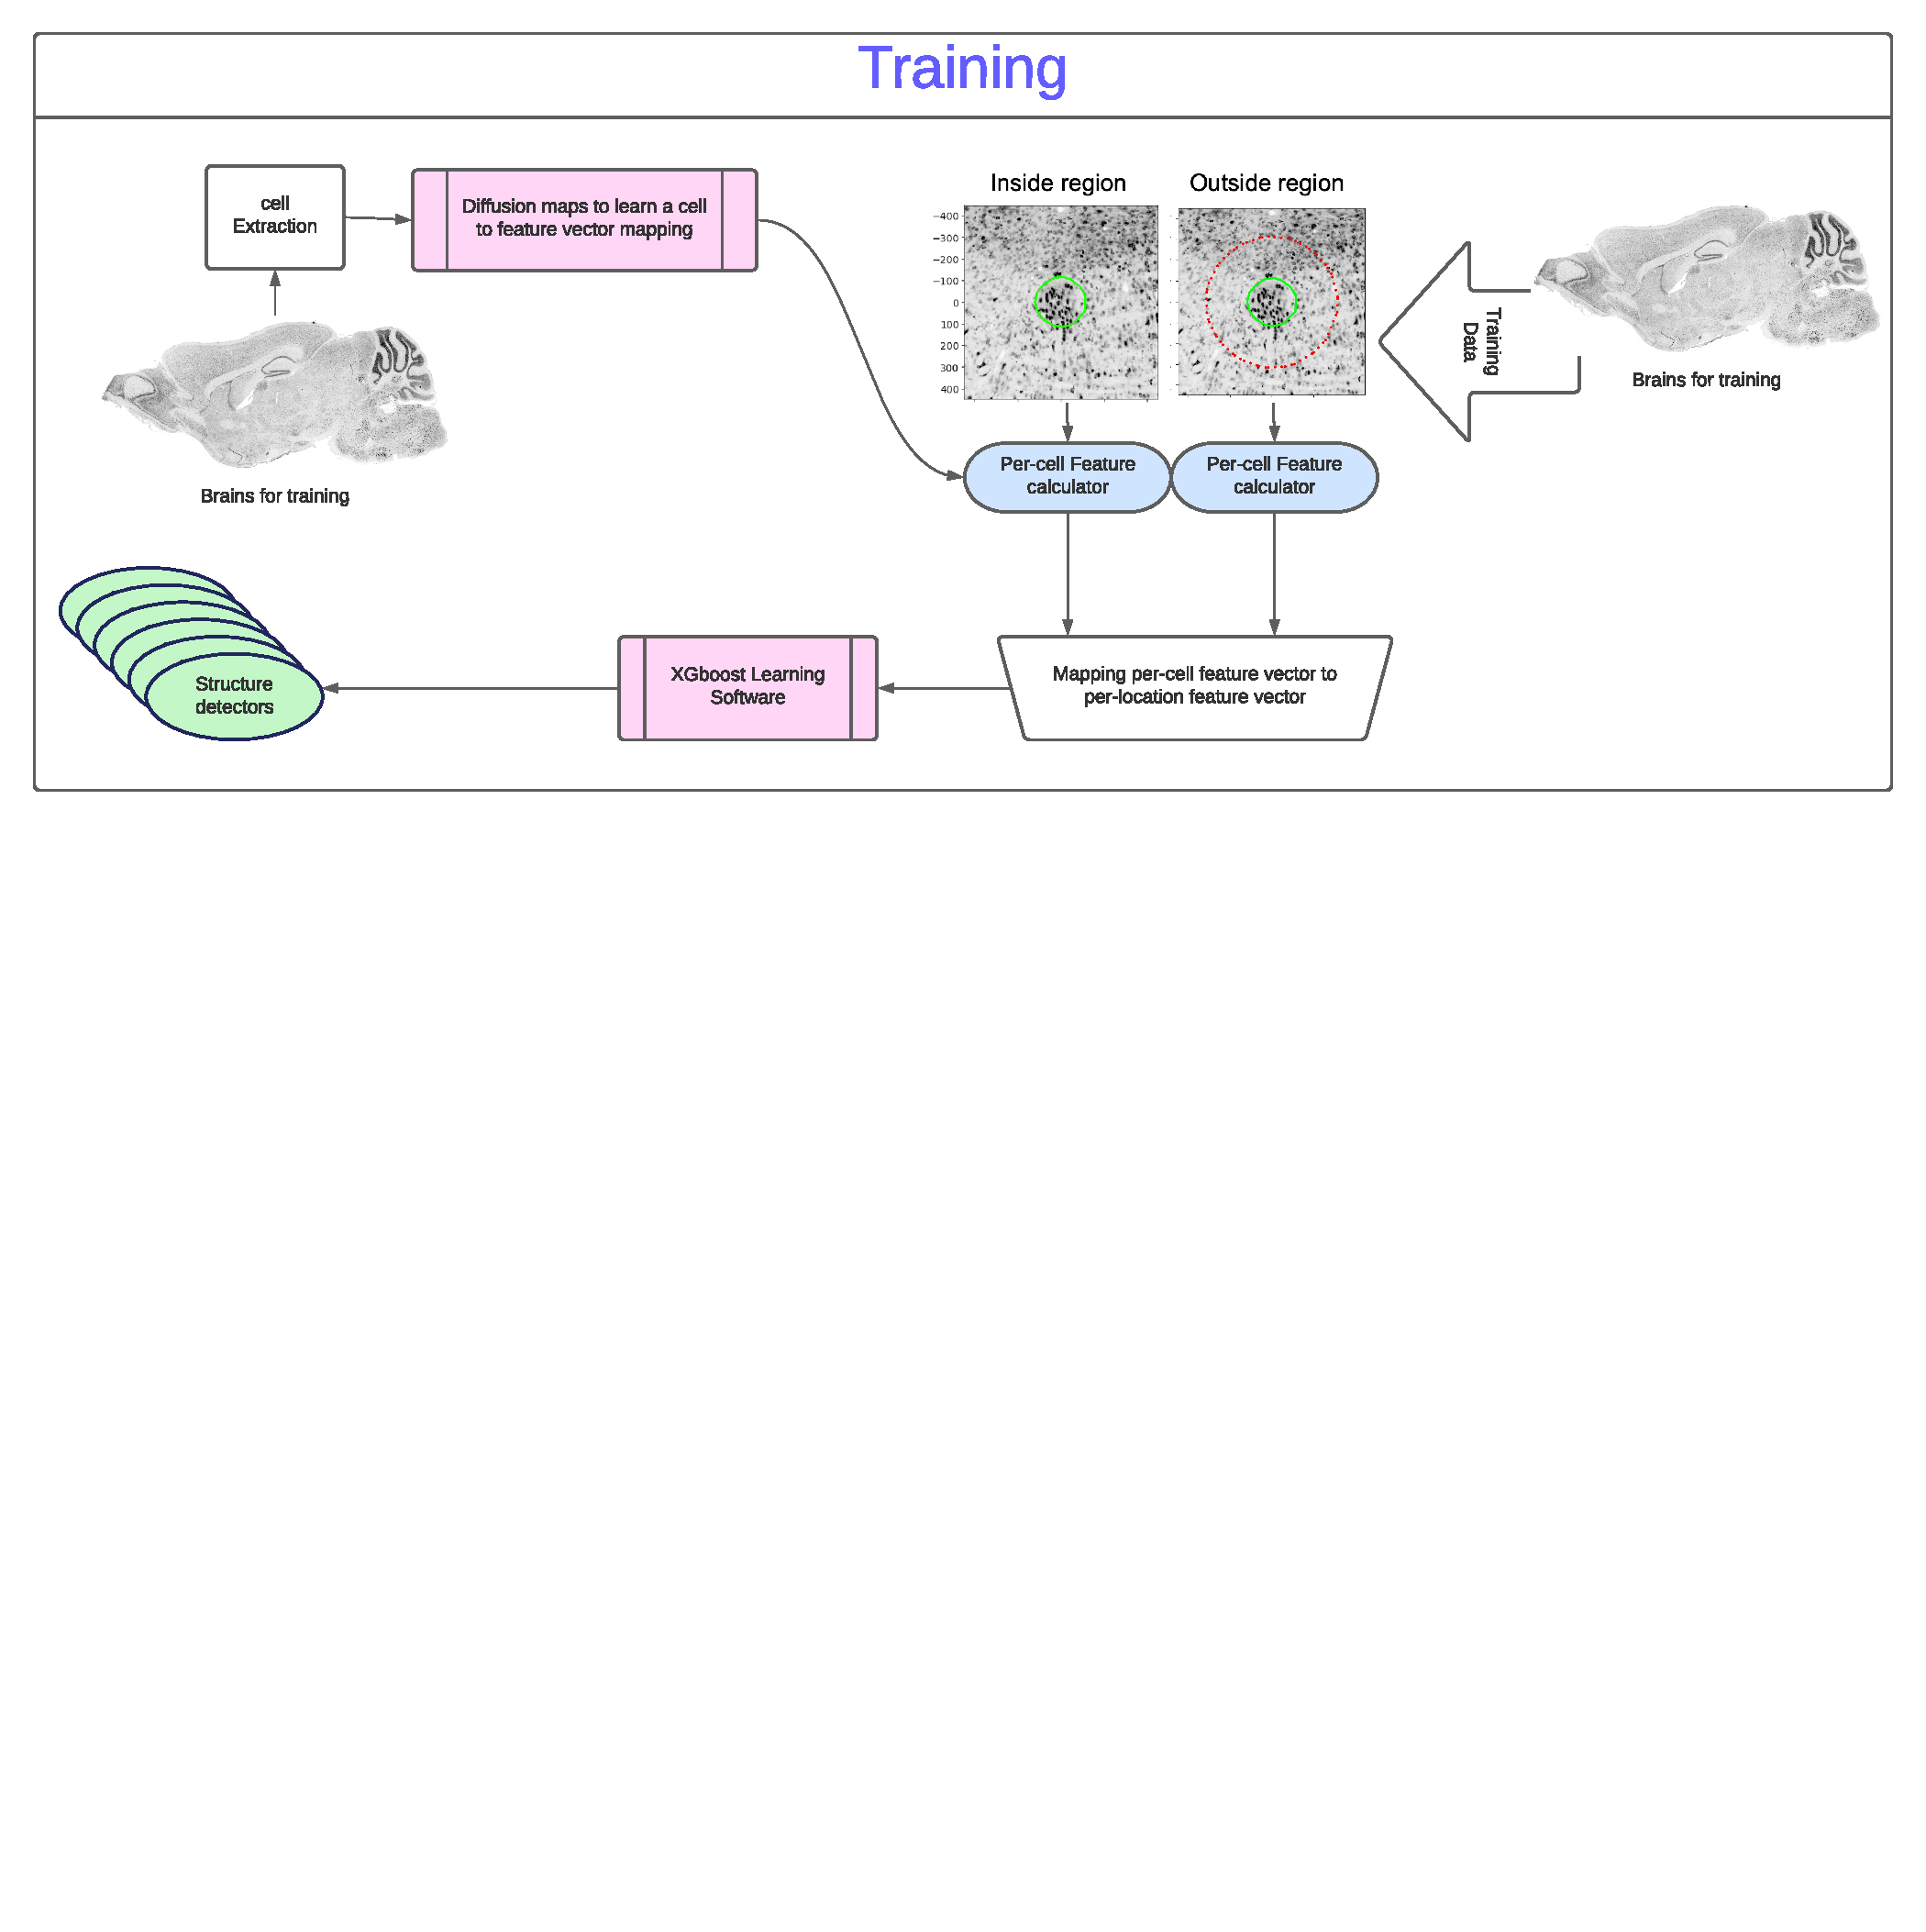
\includegraphics[width=0.6\textwidth]{figures/Training.pdf}
\caption{Training \label{fig:training}}
\end{wrapfigure}



\subsubsection { Structure detection explanation}

\iffalse
which is based on cells as the basic unit. Doing so provides an explanation for the detector's decision. We use unsupervised learning to find a dimensionality reducing mapping for cell shapes. We make efficient use of manual annotations by estimating the shape of each structure from a few brains and anatomists. We leverage this information in the detector training by having the anatomist identify the location of the center of mass for each structure.
\fi
\section{Results}
\begin{itemize}
    \item Detection results, with confidence levels, consistency with Beth.
    \item {\bf Explaining detections} The explanation of the detection is expressed in terms of cells whose shape gives evidence to the structure.
\item {\bf Cell shape parametrization} Uses a combination of Hu moments and dimensionality reduction using eigen-maps.
\begin{itemize}
    \item Eigen-maps learn a dimensionality reducing mapping cell shape to a ten dimensional representation.
    As it is an unsupervised method it requires no human labeling. We take advantage of the very large number of cells in single brain.
    \item Each brain creates a different mapping, however, the mappings can be made consistent by adding a linear transformation. This creates a stable parametrization and makes the detections more consistent.
\end{itemize}

\end{itemize}

\section{Methods}
In this section we provide more details on the algorithms we use in
our system. The full code is available from github...

\begin{itemize}
\item Cell based features.
\item Diffusion mapping.
\item Calibration of the diffusion features.
\item Region features and CDFs.
\item Boosting and XGBoost.
\item Localizing structures. Rough alignment, computing detections
  scores, computing autocorrelation and asigning confidence.
\item Using the system for brain-to-atlas alignment.
\item Generating explanations.
\end{itemize}

\section{Unplaced figures}

\begin{figure}[t]
  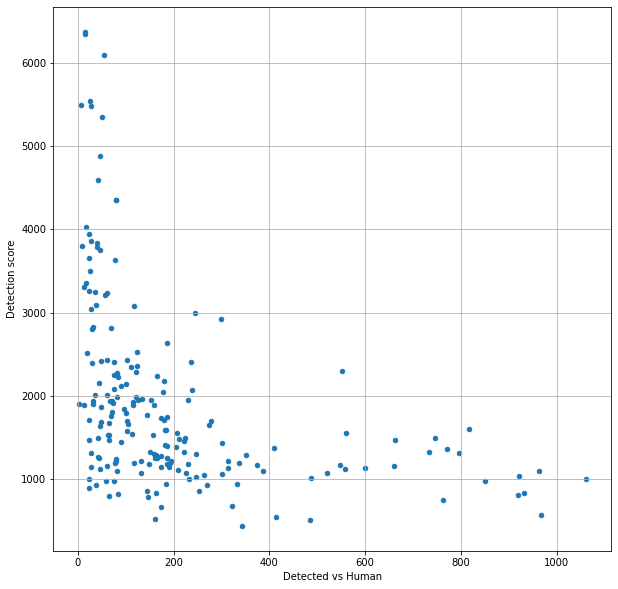
\includegraphics[width=\textwidth]{figures/DetectionConfidenceVsError.png}
  \caption{}
\end{figure}

\begin{figure}[t]
  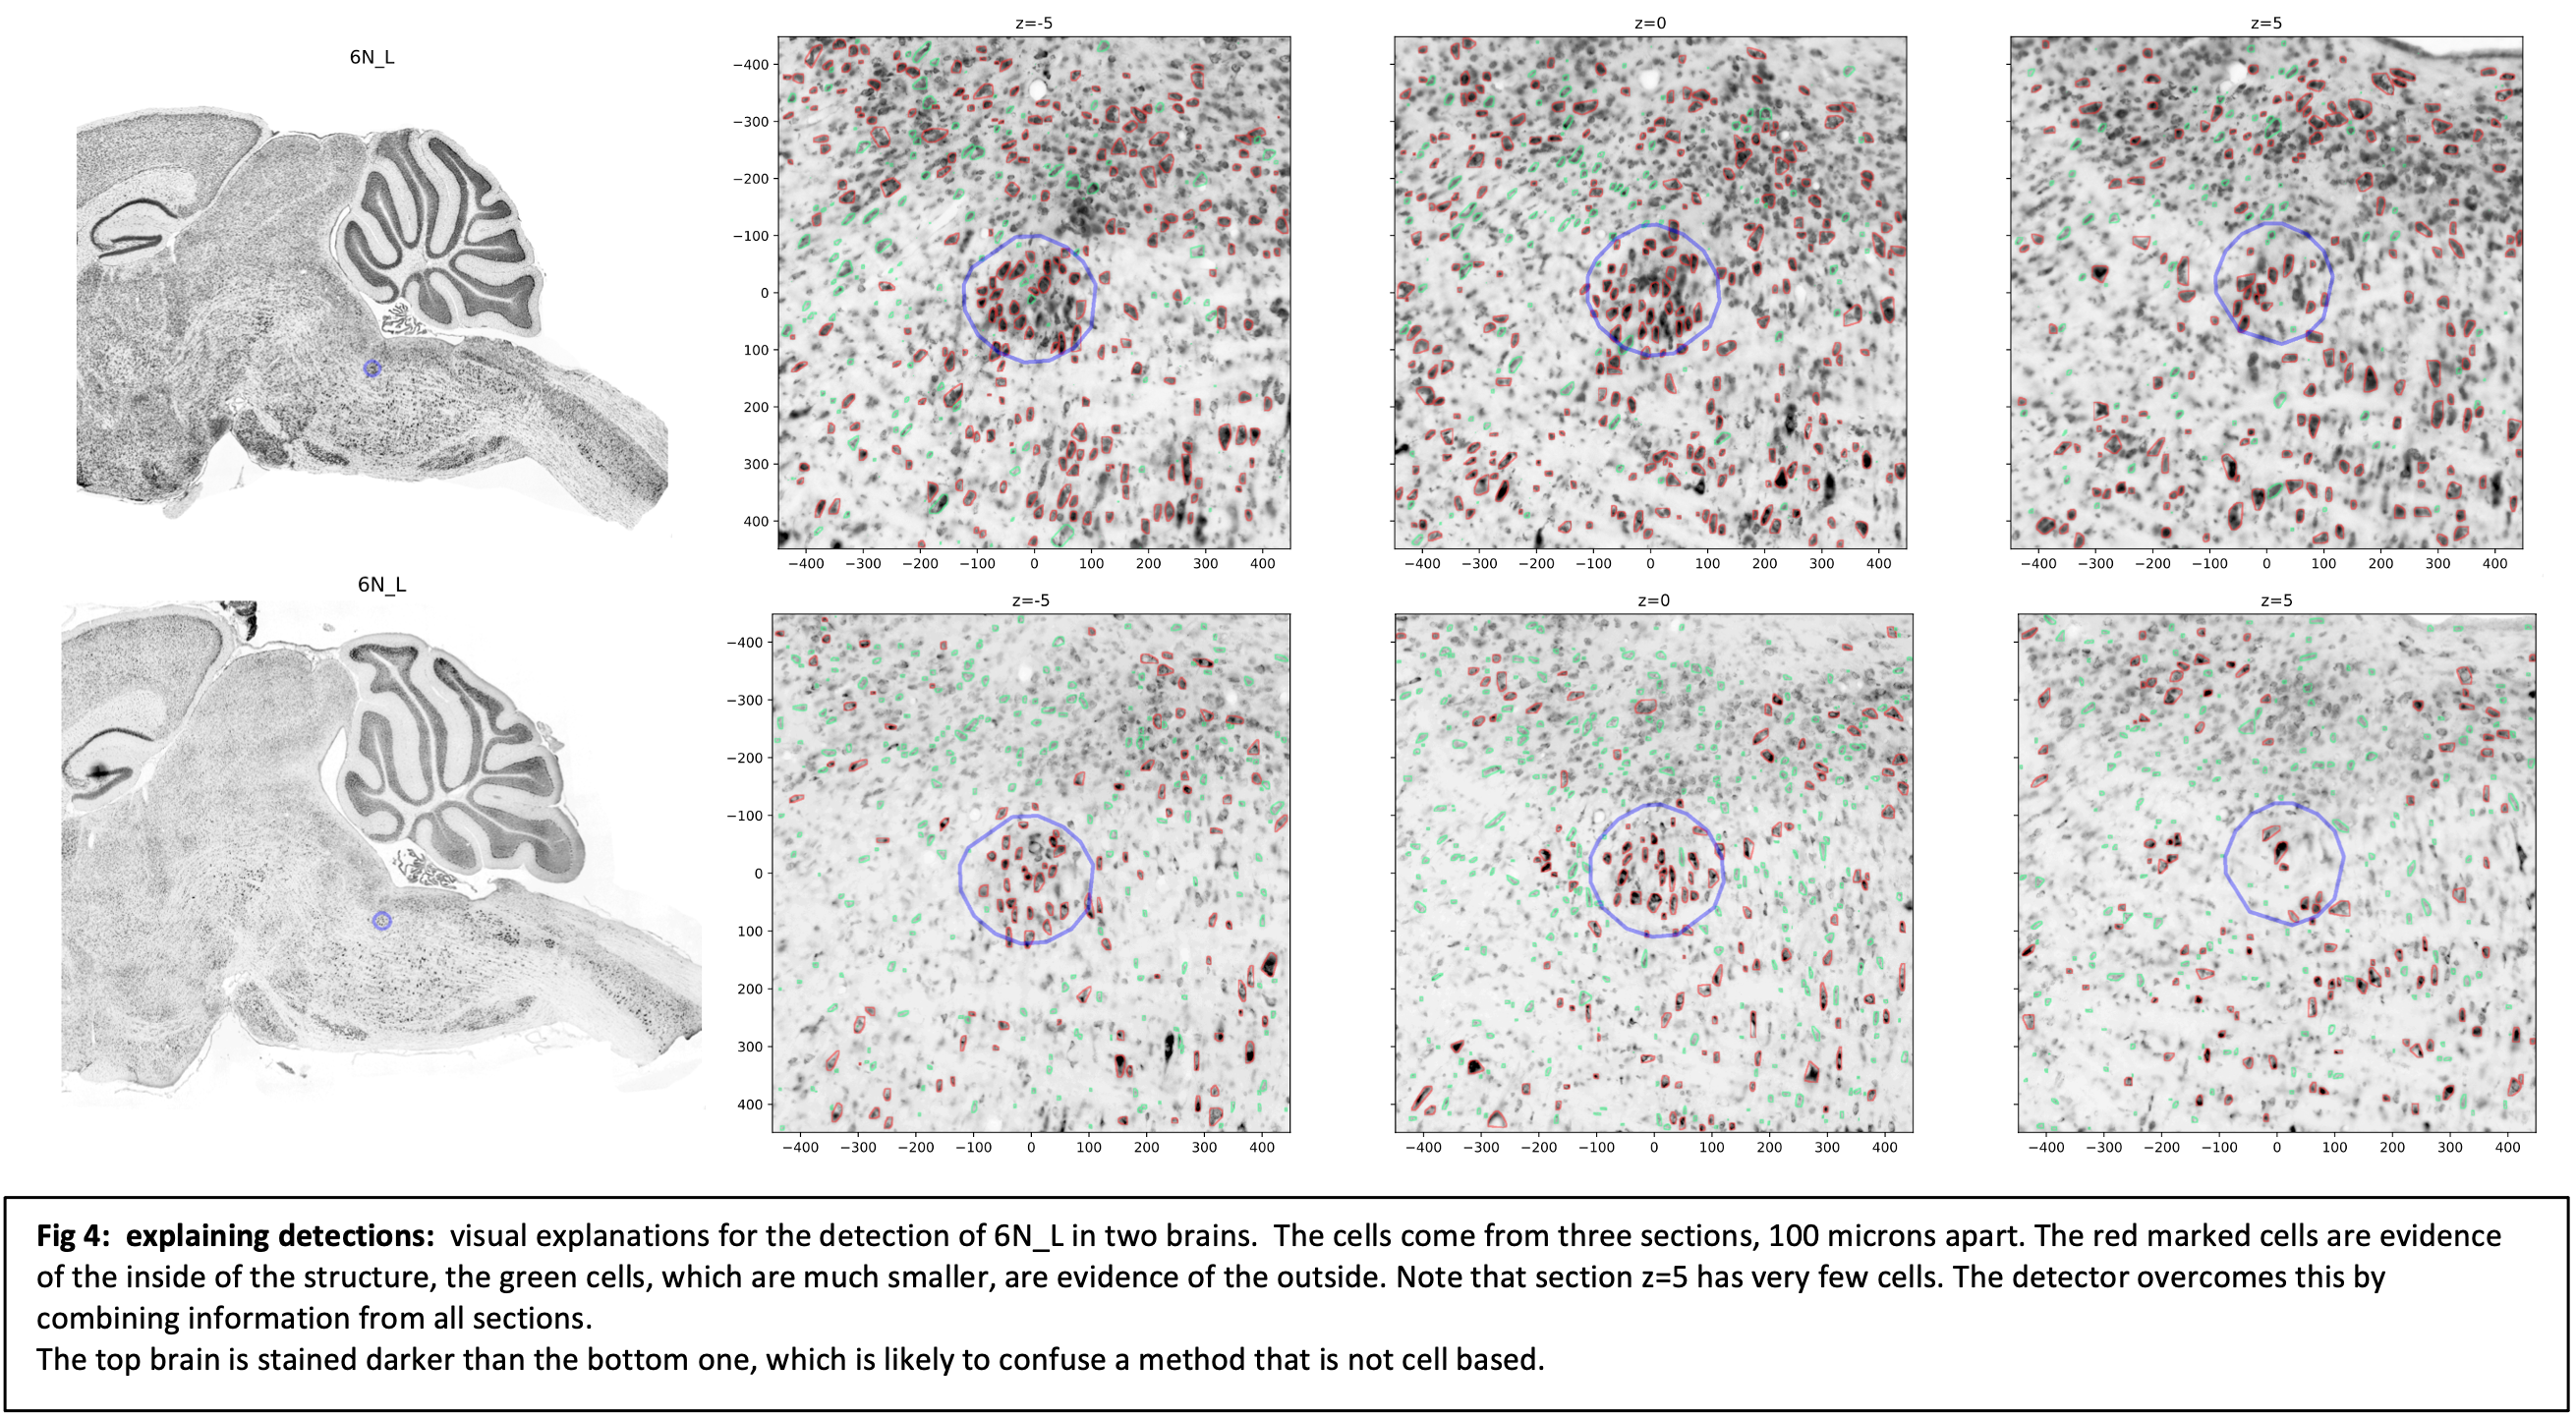
\includegraphics[width=\textwidth]{figures/DetectionsExplanations.png}
  \caption{}
\end{figure}

\begin{figure}[t]
  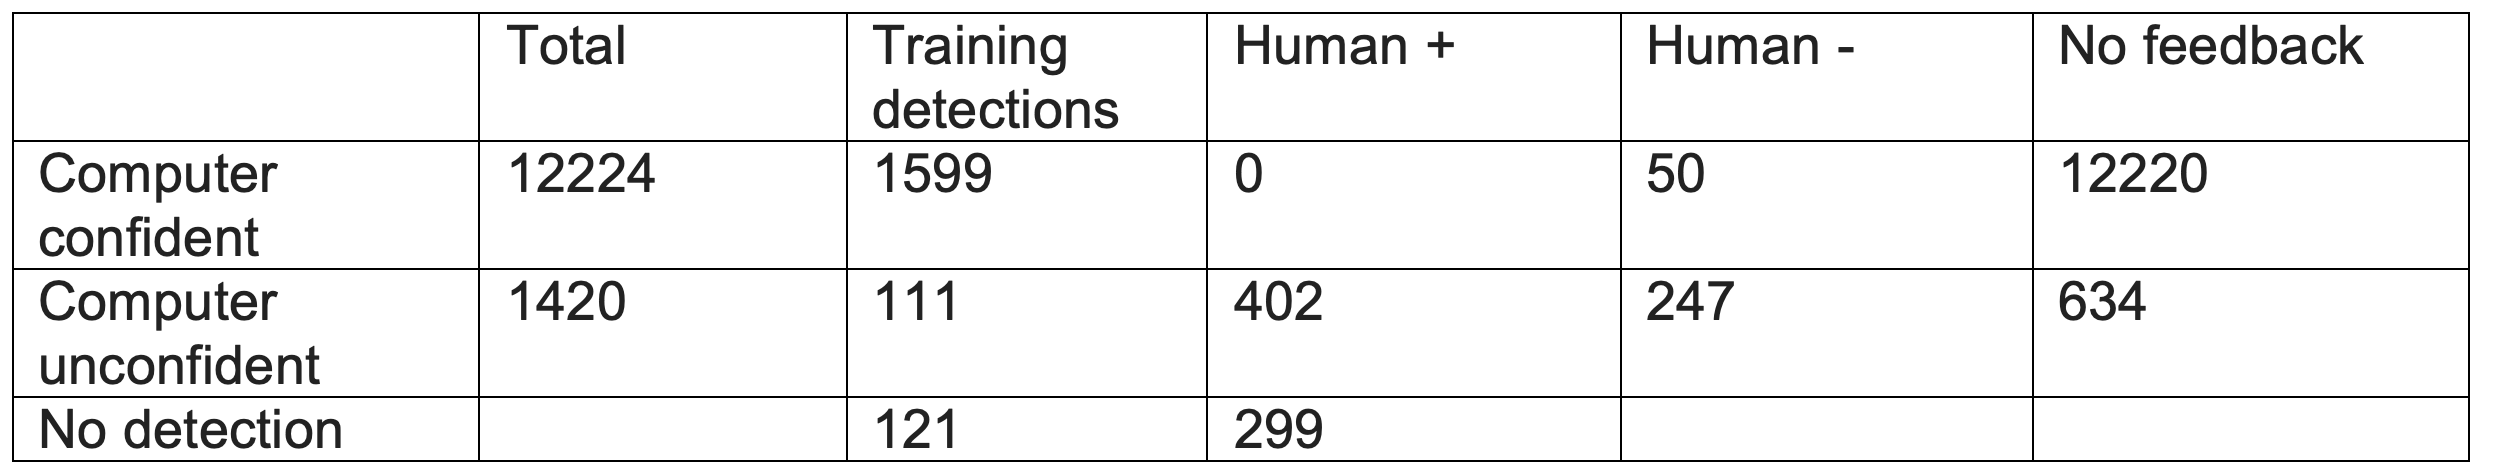
\includegraphics[width=\textwidth]{figures/MarkedCellsDetectionNumbers.png}
  \caption{}
\end{figure}

\begin{figure}[t]
  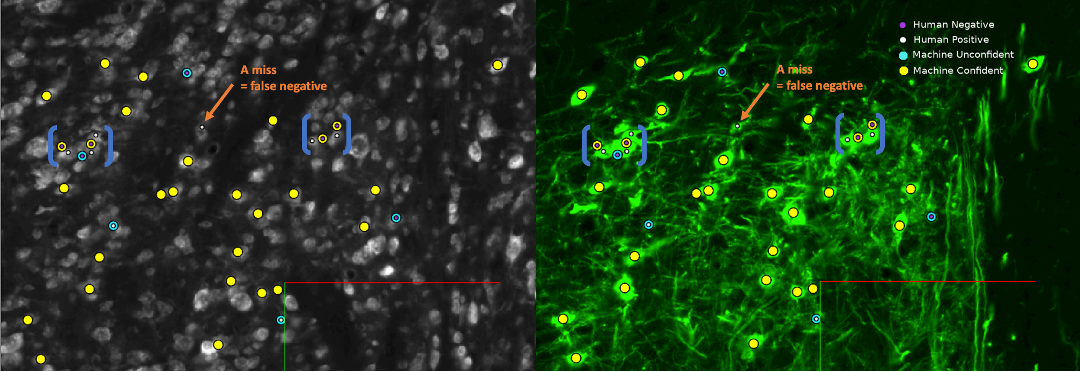
\includegraphics[width=\textwidth]{figures/Marked_cell_detections.png}
  \caption{}
\end{figure}

\begin{figure}[t]
  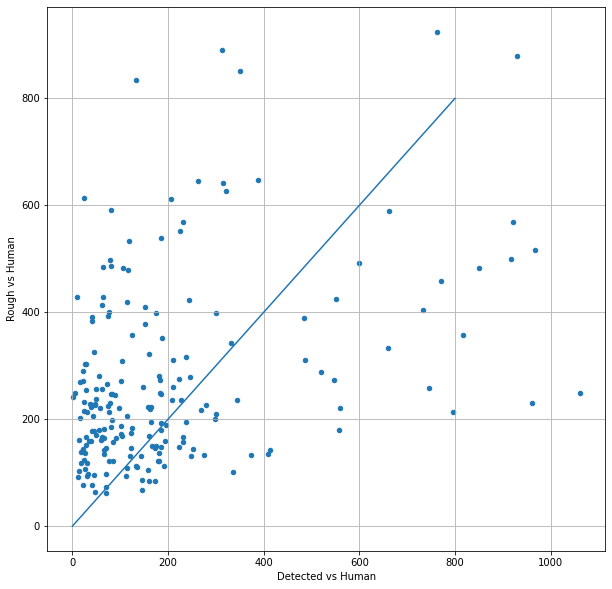
\includegraphics[width=\textwidth]{figures/RoughVSDEtection.png}
  \caption{}
\end{figure}

\begin{figure}[t]
  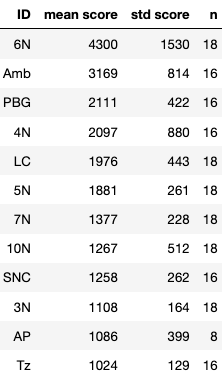
\includegraphics[width=\textwidth]{figures/ScoresOfStructures.png}
  \caption{}
\end{figure}

\end{document}


